\section{Methodology}
\label{sec:methodology}

This section outlines the research questions and analytical methods.
% Shorten
%The evaluation combines controlled experiments on ten IoT devices capturing update traffic with retrospective dataset analysis, supporting both internal and external validity.




\paragraph{Research Questions}
Guided by the objectives of this study, we focus on addressing the following  research questions (RQs):
\textbf{RQ1:}
    What are the update process characteristics of modern household IoT devices, specifically: what network protocols are used, which organizations supply the update infrastructure, and which countries host the contacted update servers?
    %, including countries.
\textbf{RQ2:}
    How trustworthy is the update delivery channel of IoT devices: specifically, do devices authenticate update servers to ensure firmware authenticity, and do they adequately protect firmware confidentiality through strong encryption and secure cryptographic configurations?
\textbf{RQ3:}
    What security implications arise when update channels use weak or insecure cryptographic configurations, and what known vulnerability classes are associated with those configurations?

   % \item[\textbullet] \textbf{RQ4:}
    %From which countries do IoT devices receive software updates?



\subsection{Threat Model}
\label{subsec:threat_model}


We consider a smart home deployment in which IoT devices periodically retrieve software or firmware updates from remote vendor servers over the Internet. 
The update channel traverses one or more intermediate network segments.
%(e.g., the local Wi-Fi link, the home gateway, and upstream ISP or cloud infrastructure).

\paragraph{Adversary profile}
We assume a network-level adversary ($\mathcal{A}$) who can passively observe traffic on any segment of the update path. 
Specifically, $\mathcal{A}$ may be (i)~an on-path Wi-Fi eavesdropper within range of the home access point, (ii)~a compromised or backdoored home gateway or router, or (iii)~a transit-level observer (e.g., a compromised ISP node or a state-level actor).
In the passive setting, $\mathcal{A}$ can capture packet metadata (sizes, timing, directions, IP addresses, and DNS queries) as well as any cleartext payload transmitted over unencrypted channels (HTTP).
Under an active extension, $\mathcal{A}$ can additionally inject, modify, or replay packets, enabling man-in-the-middle, TLS downgrade, and update substitution attacks when weak or insecure cryptographic configurations are present.

\paragraph{Adversary goals}
The adversary pursues the following objectives:
\emph{Reconnaissance:} Fingerprint device types and infer firmware versions by analyzing update-related traffic patterns %(contacted endpoints, payload sizes, and protocol metadata), 
enabling pre-exploitation target prioritization.
\emph{Confidentiality violation:} Extract sensitive information from update traffic, such as version metadata or configuration data, particularly when transmitted over unencrypted channels (HTTP) or protected by weak cipher suites.
    %identified in our analysis.
\emph{Integrity violation:} Tamper with or substitute firmware binaries during transit by exploiting weak or insecure TLS configurations (e.g., cipher suites susceptible to downgrade attacks).
    %, potentially achieving persistent code execution on the device.
\emph{Authenticity violation:} Impersonate a legitimate update server by exploiting weak certificate configurations (e.g., short-lived key lengths below the NIST 128-bit security threshold) to deliver malicious firmware undetected.

\paragraph{Trust assumptions}
We assume that the vendor's update server itself is not compromised. 
We further assume that the IoT device firmware, at the time of deployment, is authentic. The security of the update \emph{delivery channel} between the server and the device is \emph{not} assumed and is the subject of our analysis.


























\subsection{Controlled Experiments}

We conducted controlled experiments using ten heterogeneous smart IoT devices. For each device, software update processes were initiated under controlled laboratory conditions. During these update procedures, network traffic was recorded using Wireshark and \texttt{tcpdump}. 
%(e.g., \texttt{sudo tcpdump -i wlan0 -w traffic/apple-tv.pcapng}).
%The devices used for the controlled experiments are apple-tv, sony-tv, fire-tv-stick,  homepod-mini, d-link, tapo-c100, tapo-c200, eufy, xiaomi, reolink cameras,
The devices 
%for the controlled experiments 
were selected to represent diverse IoT categories: \textbf{streaming devices},
%(apple-tv, fire-tv, sony-tv), 
\textbf{smart assistants}, 
%(homepod-mini), 
and \textbf{network cameras} (Figure~\ref{fig:devices}, Appendix~\ref{app:app}). 
%(tapo-c100, tapo-c200, eufy-cam, d-link-cam, reolink-cam, xiaomi-cam),  
%as shown in Figure~\ref{fig:devices}, Appendix \ref{app:app}.
%This heterogeneity allows assessment of how device function and manufacturer design choices influence encryption practices.
The controlled experiment  consists of three main steps as shown in Figure \ref{fig:controlled_sytem_model}: 
(i) update initialization, (ii) acquisition and installation, and (iii) data collection.
First, the user agent triggers the update via mobile apps or a computer. 
Then the software update is checked, downloaded, and installed on the dedicated smart IoT device.
During steps one and two, the traffic is recorded using a Raspberry Pi 4 configured as a bridged
wireless access point \cite{raspi-config}.









\begin{figure}[!htbp]
    \centering
    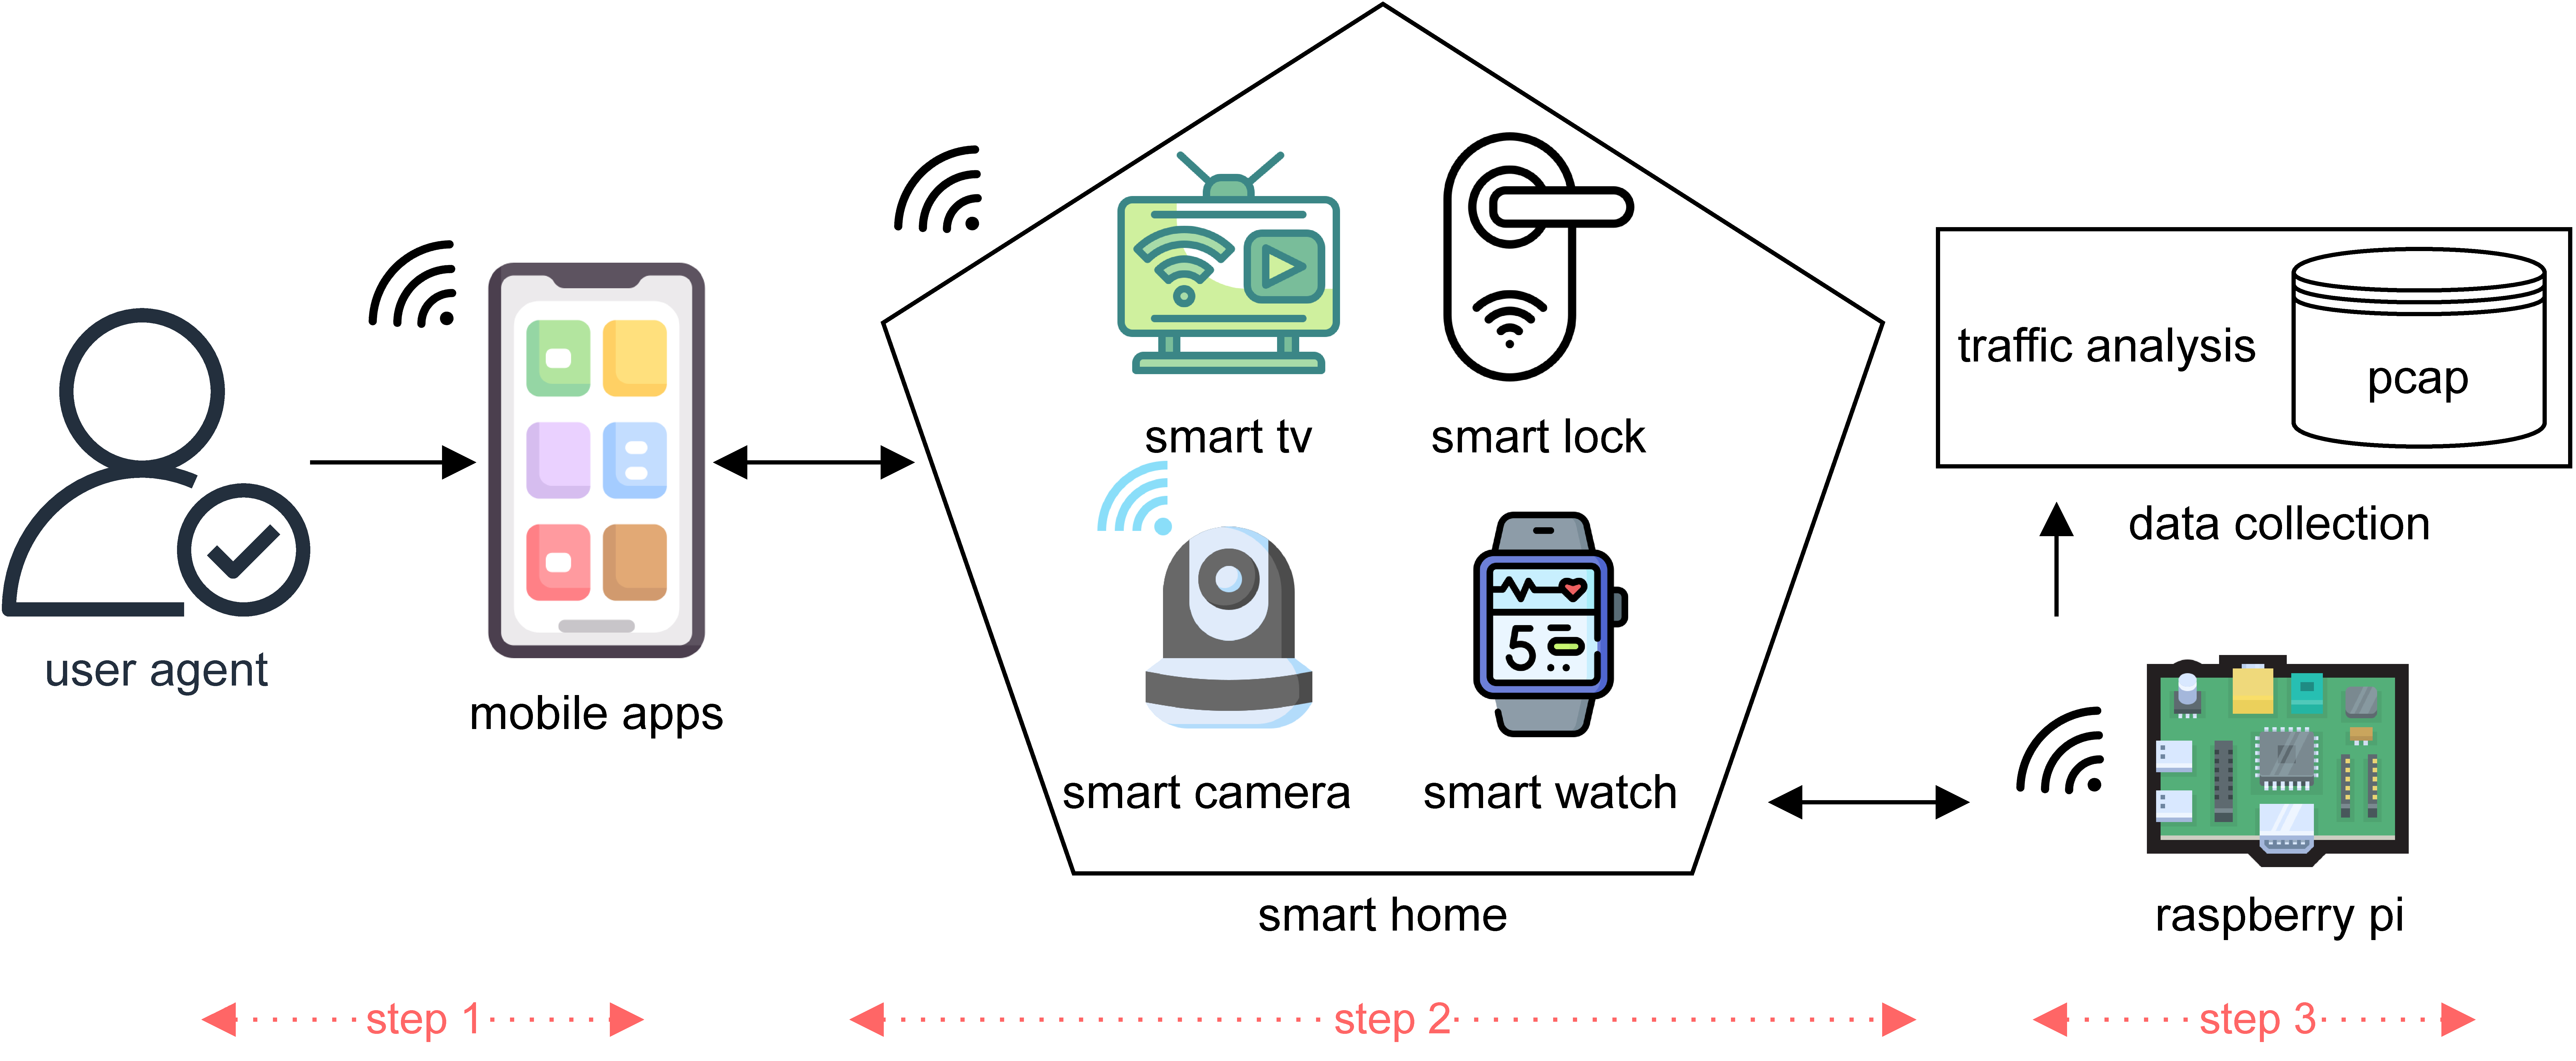
\includegraphics[width=.85\linewidth]{fig/system_setup.pdf}
    \caption{Controlled experiments setup.}
    \Description{Three-step diagram. Step 1: a user agent triggers the update through mobile apps. Step 2: smart home devices, such as a smart TV, smart lock, smart camera, and smart watch, retrieve and install the update over Wi-Fi. Step 3: a Raspberry Pi acting as the wireless access point records the traffic as pcap files for traffic analysis.}
    \label{fig:controlled_sytem_model}
\end{figure}








\subsection{Retrospective Experiments}
In addition to controlled experiments,  we conducted retrospective experiments using previously collected network traffic datasets containing IoT communication traffic.
The dataset used was generated from the Mon(IoT)r Testbed \cite{10.1145/3355369.3355577}, a large-scale IoT experimentation platform. 
The testbed comprises 81 different IoT devices (26 unique models) deployed in the US and the UK, from which 34,586 manually controlled and automated experiments were conducted. 
%The devices span several IoT categories, including cameras, smart hubs, home automation systems, televisions, audio devices, and applications.
To identify the update process characteristics from the retrospective experiments, 
we use update-related keywords, namely  \texttt{software, firmware, update,} and \texttt{download}. 
Matching traffic may signal that an update has been triggered, retrieved, and/or installed on the device. 
%Shorten:
%We selected this dataset because it is not assumed to contain any form of cyberattacks, similar to our controlled dataset, which allows us to investigate network traffic under normal operating conditions.
Based on the update-related traffic observed in the retrospective experiments, we selected the top ten update-related IoT devices for comparison with our controlled experiments.









\subsection{System Model}
We develop a system model for network traffic analysis, similar to the study in \cite{10.1007/978-3-031-30122-3_25},  consisting of three main phases: (i) data preprocessing, (ii)  metadata extraction, and  (iii) parallel execution, as shown in Figure \ref{fig:retrospective_sytem_model}.






In the data preprocessing phase, we use both our dataset from the controlled experiments and the dataset from the retrospective experiments \cite{10.1145/3355369.3355577}.
For the retrospective experiments dataset, we combine it as a whole, without distinguishing between geographic locations or controlled versus uncontrolled experiments, as conducted in the original study \cite{10.1145/3355369.3355577}, this approach is intended to ensure a vendor-agnostic system.
In the metadata extraction phase, we process the packet captures from the dataset, focusing on session-level information relevant to IoT device network traffic.
In the parallel execution phase, metadata extraction is parallelized and deployed on worker nodes, allowing packets to be processed consecutively. 
% shorten
%This parallel pipeline supports efficient network traffic management for object extraction and is designed to be compatible with distributed data processing technologies, such as Apache Hadoop \cite{10.1007/978-3-031-30122-3_25}.
As part of this process, we filter metadata using the aforementioned update-related keywords
%, namely \texttt{software, firmware, update}, and \texttt{download} 
for the retrospective experiments, to extract update-related network traffic.
The final phase of the system model involves distinguishing encrypted from unencrypted network traffic by extracting HTTPS protocol sessions that include the TLS handshake and HTTP protocol sessions, respectively.
This process involves using and modifying the PyShark to disassemble the client and server hello for the TLS handshake, which allows us to reveal, among other things, the entropy, the TLS version, and the cipher suites information.
% the handshake type, 
The results
%of this process 
are stored as extractable metadata in a database, making them ready for further processing in the analysis pipeline, and the encrypted and unencrypted analysis outcomes are retained on the file system.












\begin{figure}[!htbp]
    \centering
    \includegraphics[width=\linewidth]{fig/model.pdf}
    \caption{System model for traffic analysis.}
    \Description{Pipeline diagram. Packet captures from the controlled experiment and from the retrospective experiment, whose metadata is extracted per application, region, and device, flow into a parallel execution environment. There, PyShark worker nodes filter packets with the keywords software, firmware, update, and download, then parse TLS handshakes and extract HTTP objects. Results are written to the file system and as JSON metadata files.}
    \label{fig:retrospective_sytem_model}
\end{figure}




\subsection{Entropy Analysis}
To quantify the uncertainty or randomness in encrypted traffic payloads, we compute three types of entropy: \texttt{Shannon, Rényi}, and \texttt{Tsallis} \cite{6088496},
following the approach in \cite{10.1145/3355369.3355577}. These measures provide different perspectives on the distribution of byte-level frequencies, helping to capture subtle structural differences in encrypted data.

The \texttt{Shannon} entropy is the most widely used measure of information content. For a discrete random variable $X$  with probability distribution ${\{ p_1, p_2, \ldots, p_n \}}$, the Shannon entropy is defined as:
$
    H_{\text{Shannon}}(X) = - \sum_{i=1}^{n} p_i \log_b(p_i)
$,
where $p_i$ is the probability of the $i$-th byte value in the packet payload, and $b$ is the base of the logarithm (in our case, $b=256$ to match the byte range). This entropy quantifies the average uncertainty. %or surprise in observing byte values.
The \texttt{Rényi} entropy is a generalization of Shannon entropy that introduces a tunable parameter $\alpha$ to control the sensitivity to different probability magnitudes:
For order \( \alpha > 0 \) and \( \alpha \ne 1 \):
$
H_{\text{Rényi}}^{(\alpha)}(X) = \frac{1}{1 - \alpha} \log_b \left( \sum_{i=1}^{n} p_i^{\alpha} \right)
$.
When $\alpha \to 1$, Rényi entropy converges to Shannon entropy. Lower values of $\alpha$ emphasize more uniform distributions, while higher values give more weight to dominant probabilities. In our experiments, we use $\alpha = 2$.
The \texttt{Tsallis} entropy is another generalization of Shannon entropy, widely used in non-extensive statistical mechanics. 
In this set-up,
for order \( q > 0 \) and \( q \ne 1 \):
$
H_{\text{Tsallis}}^{(q)}(X) = \frac{1}{q - 1} \left(1 - \sum_{i=1}^{n} p_i^q \right)
$.
Here, $q$ is a real parameter (with $q   \neq 1$), and as $q \to 1$, the formula also reduces to Shannon entropy. Tsallis entropy emphasizes contributions from rare events differently from Rényi entropy, making it useful for capturing tail behavior in the distribution.
In our experiments, we use $q = 1.5$. All three measures are normalized to the $[0,1]$ range for cross-device comparability.








\subsection{Cipher Suites Identification}
\label{subsec:cipher_method}
To analyze the cryptographic mechanisms used during update sessions, we extracted cipher suites information from observed TLS handshakes.
Each cipher suite was represented in its raw 16-bit hexadecimal identifier (as it appears in the handshake).
To enable consistent comparison across devices, versions, and library implementations, these values were then normalized using the IANA TLS cipher suites registry
\cite{IANA_parameters}, which provides a canonical mapping from numeric identifiers to standardized cipher suites names. An example of these names is
\texttt{0xC05C} $\rightarrow$
\path{TLS\_ECDHE\_ECDSA\_WITH\_ARIA\_128\_GCM\_SHA256}.
%Converting cipher suites communication between clients and server from hexadecimal to IANA.



\paragraph{Classification criteria}
Each normalized suite is assigned to one of four categories (insecure, weak, secure, and recommended) based on the community benchmark of \path{ciphersuite.info}, following IETF and NIST guidance \cite{NIST2020-SP800-57}.
The criteria are provided in Table~\ref{tab:cipher_classification}.
\emph{Insecure:} broken suites using obsolete primitives (e.g., NULL, EXPORT, RC4, DES/3DES, anonymous key exchange, or MD5) that should never be used.
\emph{Weak:} deprecated suites relying on outdated primitives, CBC, static RSA, or SHA-1, vulnerable to downgrade, padding-oracle, and retrospective-decryption attacks.
\emph{Secure:} state-of-the-art AEAD-based suites with no known practical attacks, though they may lack forward secrecy.
\emph{Recommended:} TLS~1.3-grade AEAD suites with Perfect Forward Secrecy via ephemeral (EC)DHE, providing the strongest security for modern deployments.

\begin{table}[!htbp]
    \centering
    \caption{Cipher suite classification criteria and  adversarial capability, following the \texttt{ciphersuite.info} benchmark and IETF/NIST~\cite{NIST2020-SP800-57} guidance. AEAD: authenticated encryption with associated data; PFS: (perfect) forward secrecy via ephemeral (EC)DHE.}
    \label{tab:cipher_classification}
    \setlength{\tabcolsep}{3pt}
    \resizebox{\linewidth}{!}{%
    \begin{tabular}{@{} l | >{\raggedright\arraybackslash}p{3.5cm} | >{\raggedright\arraybackslash}p{4.05cm} | >{\raggedright\arraybackslash}p{3.6cm} @{}}
    \toprule
    \textbf{} & \textbf{Defining criteria} & \textbf{Representative suites} & \textbf{Adversarial capability} \\ \hline
    \textbf{Insecure} & Broken primitives: NULL, EXPORT, RC4, DES/3DES, MD5 or anonymous key %exchange 
    & \texttt{RSA\_RC4\_128\_MD5}, \texttt{DH\_anon}, NULL/EXPORT suites & Passive plaintext recovery, MITM/impersonation, key recovery \\ \hline
    \textbf{Weak} & Deprecated primitives: CBC record protection, static RSA (no PFS), or SHA-1 & \texttt{ECDHE\_RSA\_AES\_256\_CBC\_SHA}\newline \texttt{RSA\_AES\_128\_CBC\_SHA} & Padding-oracle (BEAST/Lucky13), downgrade, no-PFS retrospective decryption \\ \hline
    \textbf{Secure} & AEAD with no known practical attack, but may lack PFS & \texttt{ECDHE\_ECDSA\_AES\_128\_CCM}\newline static-RSA AES-GCM suites & Retrospective decryption only if the long-term key later leaks (no PFS) \\ \hline
    \textbf{Recommended} & AEAD \emph{and} PFS; TLS~1.3 -grade (e.g., ECDHE with AES-GCM or ChaCha20) & \texttt{TLS\_AES\_128\_GCM\_SHA256}\newline \texttt{ECDHE\_RSA\_AES\_256\_GCM} & None passively; PFS limits the impact of long-term key compromise \\
    \bottomrule
    \end{tabular}%
    }
\end{table}




%Shorten
%\textbf{Offered vs. negotiated suites.}
%A TLS \texttt{ClientHello} advertises the full list of suites a client is \emph{willing}
%to use, whereas the \texttt{ServerHello} records the single suite actually \emph{negotiated}
%for the session. We analyzed these separately throughout: \texttt{ClientHello} lists are
%treated as capability/offer data that bound a device's downgrade \emph{exposure}, while
%negotiated cipher strength and TLS version are taken from the \texttt{ServerHello}
%(handshake type~2). Conflating the two would overstate weakness, because a client may
%advertise legacy suites that are never selected; keeping them distinct lets us
%distinguish residual capability from realized cryptographic posture.







\subsection{Certificate Security Analysis}
Server authentication in TLS relies on X.509 certificate validation; the entropy and cipher suite analyses that follow characterize how well the channel protects firmware confidentiality once server identity is established.
We performed a multi-stage analysis of X.509 certificates across the selected IoT devices.
First, certificate files were extracted from each device's TLS sessions captured during the controlled experiments.
Second, each X.509 certificate was parsed to extract cryptographic and lifecycle metadata, including public key algorithm, key size, signature algorithm, validity interval (\texttt{notBefore}/\texttt{notAfter}), issuer and subject distinguished names, serial number, and self-signed (SS) status, following X.509 specifications \cite{rfc5280,rfc4055,rfc5480}.
Third, certificates were grouped by NIST SP~800-57 security strength\cite{NIST2020-SP800-57}: 
RSA-1024 maps to up to 80-bit security strength, 
RSA-2048 to 112-bit security strength, and RSA-3072+/EC P-256+ to at least 128-bit security strength. 
Under NIST transition guidance, strengths below 112 bits are disallowed for applying protection, 112 bits is acceptable through 2030 but disallowed for applying protection from 2031 onward (legacy use for processing), and 128 bits and above remain acceptable.
This classification enables a quantitative assessment of whether IoT vendors deploy certificates that meet contemporary cryptographic standards for securing update traffic.
Table~\ref{tab:key_size_consequences} lists the key sizes observed in our captures with their security strength and approval status.

\begin{table}[!htbp]
    \centering
    \caption{Certificate key sizes and corresponding NIST~\cite{NIST2020-SP800-57} security strength.}
    \label{tab:key_size_consequences}
    \setlength{\tabcolsep}{3pt}
    \resizebox{\linewidth}{!}{%
    \begin{tabular}{@{} l | l | l | >{\raggedright\arraybackslash}p{3.3cm} | >{\raggedright\arraybackslash}p{3.4cm} @{}}
    \toprule
    \textbf{Key} & \textbf{Algorithm} & \textbf{Strength} & \textbf{Approval status (SP~800-57, Table~4)} & \textbf{Practical consequence} \\ \hline
    256-bit  & ECC (P-256) & 128 bits       & Acceptable now and beyond 2031 & Small key; fast handshakes; ideal for IoT \\ \hline
    384-bit  & ECC (P-384) & 192 bits       & Acceptable now and beyond 2031 & Higher assurance; slightly slower than P-256 \\ \hline
    1024-bit & RSA         & $\leq 80$ bits & Disallowed for applying protection & Factorable; no protection guarantee \\ \hline
    2048-bit & RSA         & 112 bits       & Acceptable through 2030; disallowed from 2031 & Adequate today; hard expiration date \\ \hline
    4096-bit & RSA         & 128 bits       & Acceptable now and beyond 2031 & Meets target but $16\times$ larger key than ECC-256 \\
    \bottomrule
    \end{tabular}%
    }
\end{table}




\subsection{Vulnerability Analysis}


To investigate the vulnerability implications of  
%insecure and weak 
update-related traffic, we queried the CVE-List \cite{CVE_Program} database using our results derived from insecure and weak cryptographic algorithm implementations. 
To collect and curate the dataset, we followed the methods used in \cite{USMAN2026105019}. 
We search for keyword combinations including \texttt{weak}, \texttt{insecure}, and cipher suite terms.
This allows us to assess the severity of vulnerabilities and identify associated weaknesses of the insecure and weak cipher suites.
%and detail the adversarial capabilities enabled by the software update traffic flows from our cipher suites findings.
To improve traceability, we applied a deterministic mapping workflow: (i) expand each observed insecure/weak suite to canonical IANA names, aliases, and legacy names, (ii) query CVE records using Boolean combinations of protocol family (TLS/SSL), algorithm primitive (e.g., RSA, CBC, RC4, null/anonymous), and weakness terms, (iii) deduplicate by CVE-ID, and (iv) retain only records whose descriptions explicitly reference cryptographic negotiation, certificate validation, or transport-channel confidentiality/integrity weaknesses.
